\documentclass[pdflatex,compress,mathserif]{beamer}

%\usetheme[dark,framenumber,totalframenumber]{ElektroITK}
\usetheme[darktitle,framenumber,totalframenumber]{ElektroITK}

\usepackage[utf8]{inputenc}
\usepackage[T1]{fontenc}
\usepackage{lmodern}
\usepackage[bahasai]{babel}
\usepackage{amsmath}
\usepackage{amsfonts}
\usepackage{amssymb}
\usepackage{graphicx}
\usepackage{multicol}
\usepackage{lipsum}

\newcommand*{\Scale}[2][4]{\scalebox{#1}{$#2$}}%

\title{METODE NUMERIK}
\subtitle{Interpolasi Polinom}

\author{Tim Dosen Pengampu}

\begin{document}

\maketitle

\section{Pengantar}

\begin{frame}
	\frametitle{Pengantar}
	\begin{itemize}
		\item Sebuah pengukuran fisika telah dilakukan untuk menentukan hubungan antara tegangan yang diberikan kepada baja tahan-karat dan waktu yang diperlukan hingga baja tersebut patah.
		\item Delapan nilai tegangan yang berbeda dicobakan, dan data yang dihasilkan adalah
		\begin{center}
			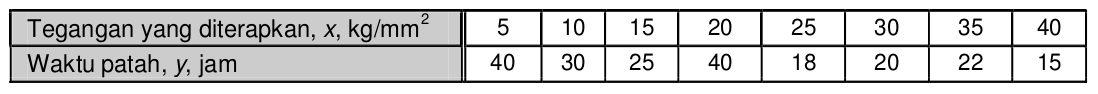
\includegraphics[width=\linewidth]{img/img01}
		\end{center}
		\item Berapa waktu patah $ y $ jika tegangan $ x $ yang diberikan kepada baja adalah 12 kg/mm$ ^2 $ .
	\end{itemize}
\end{frame}

\begin{frame}
	\begin{itemize}
		\item Solusinya dicari dengan metode pencocokan kurva (\textit{curve fitting}).
		\item Yaitu mencari fungsi yang mencocokkan (\textit{fit}) titik-titik data di dalam tabel tabel.
		\item Pencocokkan kurva adalah sebuah metode yang mencocokkan titik data dengan sebuah kurva (\textit{curve fitting}) fungsi.
		\item Pencocokan kurva dibedakan atas dua metode:
		\begin{enumerate}
			\item Regresi
			\item Interpolasi
		\end{enumerate}
	\end{itemize}
\end{frame}

\begin{frame}
	\begin{enumerate}
		\item \textbf{Regresi}
		\begin{itemize}
			\item Data hasil pengukuran umumnya mengandung derau (\textit{noise}) atau galat yang cukup berarti.
			\item Karena data ini tidak teliti, maka kurva yang mencocokkan titik data itu tidak perlu melalui semua titik.
			Kurva tersebut cukup hanya mewakili kecenderungan (\textit{trend}) titik data, yakni kurva mengikuti pola titik sebagai suatu kelompok.
		\end{itemize}
	\end{enumerate}
\end{frame}

\begin{frame}
	\begin{enumerate}
		\setcounter{enumi}{1}
		\item \textbf{Interpolasi}
		\begin{itemize}
			\item Bila data diketahui mempunyai ketelitian yang sangat tinggi, maka kurva cocokannya dibuat melalui setiap titik.
			\item Kita katakan di sini bahwa kita \textbf{menginterpolasi} titik-titik data dengan sebuah fungsi.
			\item Bila fungsi cocokan yang digunakan berbentuk polinom, polinom tersebut dinamakan \textbf{polinom interpolasi}.
			\item Pekerjaan menginterpolasi titik data dengan sebuah polinom disebut \textbf{interpolasi (dengan) polinom}.
		\end{itemize}
	\end{enumerate}
\end{frame}

\begin{frame}
	\begin{center}
		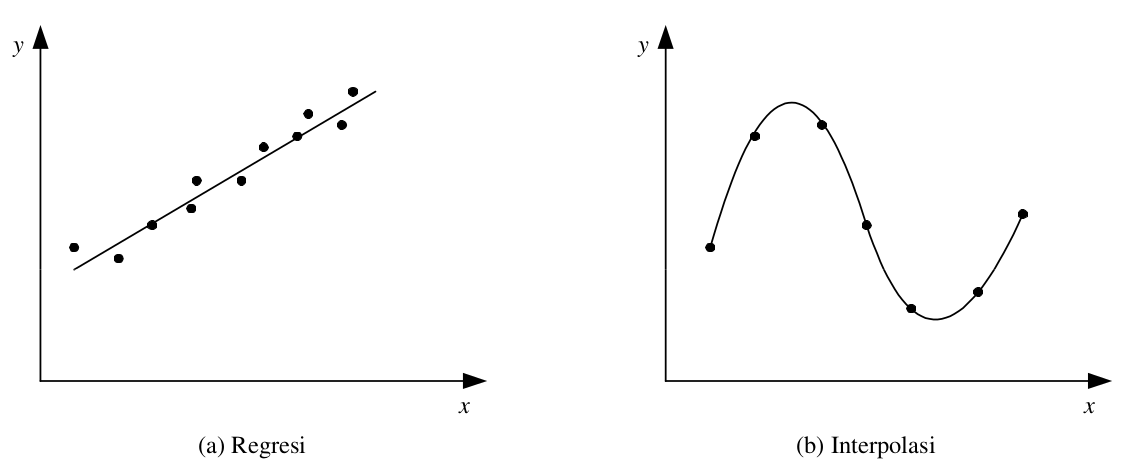
\includegraphics[width=\linewidth]{img/img02}
	\end{center}
\end{frame}

\begin{frame}
	\frametitle{Aplikasi Interpolasi Polinom}
	\begin{enumerate}
		\item Menghampiri fungsi rumit menjadi lebih sederhana
		\begin{itemize}
			\item Contoh: \[ f(x) = \frac{\ln(2x^{(1/2)}-4x^2)^3}{\sqrt{1+2x^5}} \]
			\item[] Hitung: $ f'(x) $ dan $\int f(x) dx$
			\item Perhitungan menjadi lebih mudah jika $ f(x) $ dihampiri dengan polinom $ p(x) $.
			\item Polinom $ p(x) $ diperoleh dengan menginterpolasi beberapa titik diskrit dari $ f(x) $
		\end{itemize}
		\item Menggambar kurva (jika hanya diketahui titik-titik diskrit saja)
	\end{enumerate}
\end{frame}

\section{Interpolasi Polinom}

\begin{frame}
	\frametitle{Interpolasi Polinom}
	\textbf{Persoalan}
	\begin{itemize}
		\item Diberikan $ n+1 $ buah titik berbeda, ($ x_0 $, $ y_0 $ ), ($ x_1 $, $ y_1 $ ), $\dots$, ($ x_n $ , $ y_n $ ).
		\item Tentukan polinom $ p_n(x) $ yang menginterpolasi (melewati) semua titik-titik tersebut sedemikian rupa sehingga
		\[ y_i = p_n(x_i)\qquad \text{ untuk } i = 0,1,2,\dots,n \]
		\item Nilai $ y_i $ dapat berasal dari fungsi $ f(x) $ sedemikian sehingga \[ y_i = f(x_i), \] atau, $ y_i $ berasal dari nilai empiris yang diperoleh melalui percobaan atau pengamatan.
	\end{itemize}
\end{frame}

\begin{frame}
	\begin{itemize}
		\item $ p_n(x) $ disebut fungsi hampiran terhadap $ f(x) $.
		\item Setelah polinom interpolasi $ p_n(x) $ ditemukan, $ p_n(x) $ dapat digunakan untuk menghitung perkiraan nilai $ y $ di $ x = a $, yaitu $ y = p_n(a) $.
		\item Bergantung pada letaknya, nilai $ x = a $ mungkin terletak di dalam rentang titik-titik data ($ x_0 < a < x_n $ ) atau di luar rentang titik-titik data ($ a < x_0 $ atau $ a > x_n $ ):
		\begin{enumerate}
			\item jika $ x_0 < a < x_n $ maka $ y_k = p(x_k) $ disebut \textbf{nilai interpolasi} (\textit{interpolated value})
			\item jika $ x_0 < x_k $ atau $ x_0 < x_n $ maka $ y_k = p(x_k) $ disebut nilai \textbf{ekstrapolasi} (\textit{extrapolated value}).
		\end{enumerate}
	\end{itemize}
\end{frame}

\begin{frame}
	\begin{center}
		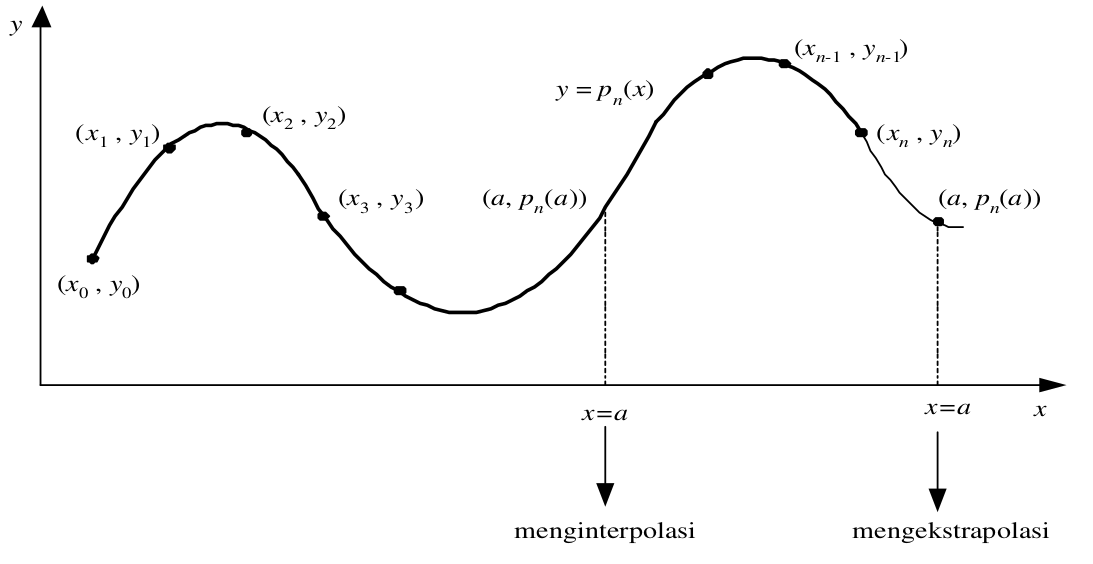
\includegraphics[width=0.7\linewidth]{img/img03}
	\end{center}
	\begin{itemize}
		\item Kita dapat menginterpolasi titik data dengan: polinom lanjar, polinom kuadratik, polinom kubik, atau polinom dari derajat yang lebih tinggi, bergantung pada jumlah titik data yang tersedia.
	\end{itemize}
\end{frame}

\subsection{Interpolasi Lanjar}

\begin{frame}
	\frametitle{Interpolasi Lanjar}
	\begin{itemize}
		\item Interpolasi lanjar adalah interpolasi dua buah titik dengan sebuah garis lurus.
		\item Misal diberikan dua buah titik, $ (x_0 , y_0) $ dan $ (x_1, y_1) $. Polinom yang menginterpolasi kedua titik itu adalah \[ p_1 (x) = a_0 + a_1 x \]
	\end{itemize}
	\begin{multicols}{2}
		\[ y_0 = a_0 + a_1 x_0;~y_1 = a_0 + a_1 x_1 \] menjadi
		\[ a_1 = \frac{y_1 - y_0}{x_1 - x_0};~a_0 = \frac{x_1 y_0 - x_0 y_1}{x_1 - x_0} \] sehingga
		\[ p_1(x) = \frac{x_1 y_0 - x_0 y_1}{x_1 - x_0} +  \frac{(y_1 - y_0)}{(x_1 - x_0)} x \]
		\columnbreak
		\begin{center}
			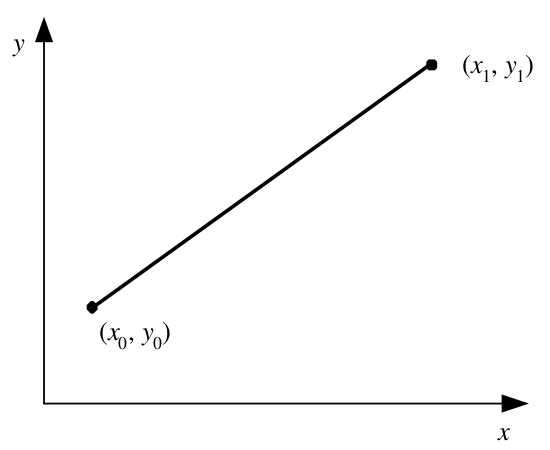
\includegraphics[width=0.8\linewidth]{img/img04}
		\end{center}
	\end{multicols}
\end{frame}

\begin{frame}
	Bila disederhanakan akan lebih lanjut:
	\begin{equation}\label{int.lanj}
		p_1(x) = y_0 + \frac{(y_1 - y_0)}{(x_1 - x_0)}(x-x_0)
	\end{equation}
\end{frame}

\begin{frame}
	\frametitle{Contoh 1}
	\begin{itemize}
		\item \textbf{Persoalan:} Perkirakan jumlah penduduk Amerika Serikat pada tahun 1968 berdasarkan data tabulasi berikut
		\begin{center}
			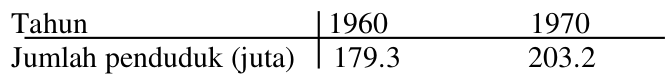
\includegraphics[width=0.8\linewidth]{img/img05}
		\end{center}
		\item \textbf{Penyelesaian:} Dengan menggunakan persamaan (\ref{int.lanj}) diperoleh
		\[ p_1(1968) = 179.3 + \frac{(203.2-179.3)(1968-1960)}{1970-1960} = 198.4 \]
		Jadi, taksiran jumlah penduduk AS pada tahun 1968 adalah 198.4 juta
	\end{itemize}
\end{frame}

\begin{frame}
	\frametitle{Contoh 2}
	\begin{itemize}
		\item \textbf{Persoalan:} Dari data $ \ln(9.0) = 2.1972 $, $ \ln(9.5) = 2.2513 $, tentukan $ \ln(9.2) $ dengan interpolasi lanjar sampai 5 angka bena. Bandingkan dengan nilai sejati $ ln(9.2) = 2.2192 $.
		\item \textbf{Penyelesaian:} Dengan menggunakan persamaan (\ref{int.lanj}), diperoleh
		\[ p_1(9.2) = 2.1972 + \frac{(2.1513-2.197)(9.2-9.0)}{9.5-90} = 2.2188 \]
		Galat = 2.2192 - 2.2188 = 0.0004. Di sini interpolasi lanjar tidak cukup untuk memperoleh ketelitian sampai 5 angka bena. Ia hanya benar sampai 3 angka bena
	\end{itemize}
\end{frame}

\subsection{Interpolasi Kuadratik}

\begin{frame}
	\frametitle{Interpolasi Kuadratik}
	\begin{itemize}
		\item Misal diberikan tiga buah titik data, $ (x_0, y_0) $, $ (x_1, y_1 ) $, dan $ (x_2, y_2) $.
		\item Polinom yang menginterpolasi ketiga buah titik itu adalah polinom kuadrat yang berbentuk:
		\begin{equation}\label{int.kuad}
			p_2(x) = a_0 + a_1x + a_2 x^2
		\end{equation}
		\begin{multicols}{2}
			\begin{center}
				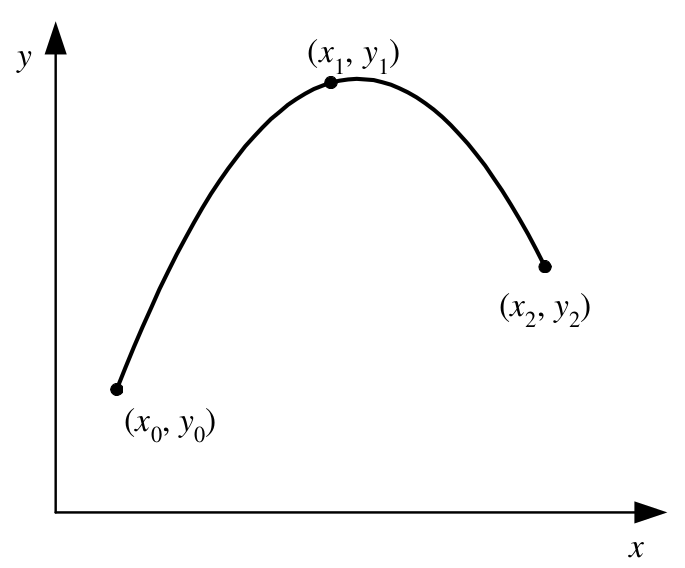
\includegraphics[width=\linewidth]{img/img06}
			\end{center}
			\item Bila digambar, kurva polinom kuadrat berbentuk parabola
		\end{multicols}
	\end{itemize}
\end{frame}

\begin{frame}{Interpolasi Kuadratik}
	Polinom $ p_2(x) $ ditentukan dengan cara berikut:
	\begin{enumerate}
		\item Sulihkan $ (x_i, y_i) $ ke dalam persamaan (\ref{int.kuad}), $ i = 0, 1, 2 $. Dari sini diperoleh tiga buah persamaan dengan tiga buah parameter yang tidak diketahui, yaitu $ a_0 $, $ a_1 $, dan $ a_2 $:
		\begin{align*}
			a_0 + a_1 x_0 + a_2 x_0^2 &= y_0\\
			a_0 + a_1 x_1 + a_2 x_1^2 &= y_1\\
			a_0 + a_1 x_2 + a_2 x_2^2 &= y_2
		\end{align*}
		\item hitung $ a_0 $, $ a_1 $, $ a_2 $ dari sistem persamaan tersebut dengan metode eliminasi Gauss.
	\end{enumerate}
\end{frame}

\begin{frame}
	\frametitle{Contoh 3}
	\begin{itemize}
		\item \textbf{Persoalan:} Diberikan titik $ \ln(8.0) = 2.0794 $, $ \ln(9.0) = 2.1972 $, dan $ \ln(9.5) = 2.2513 $. Tentukan nilai $ \ln(9.2) $ dengan interpolasi kuadratik.
		\item \textbf{Penyelesaian:} Sisten persamaan lanjar yang terbentuk adalah
		\begin{align*}
		a_0 + 8.0 a_1 + 64.00 a_2 &= 2.0794\\
		a_0 + 9.0 a_1 + 81.00 a_2 &= 2.1972\\
		a_0 + 9.5 a_1 + 90.25 a_2 &= 2.2513
		\end{align*}
		\item Penyelesaian sistem persamaan dengan metode eliminasi Gauss menghasilkan $ a_0 = 0.6762 $, $ a_1 = 0.2266 $, dan $ a_3 = -0.0064 $. Polinom
		kuadratnya adalah
		\[ p_2(x) = 0.6762 + 0.2266x - 0.0064x^2 \]
	\end{itemize}
\end{frame}

\begin{frame}{Contoh 3}
	\begin{itemize}
		\item sehingga \[ p_2(9.2) = 2.2192 \] yang sama dengan nilai sejatinya (5 angka bena).
	\end{itemize}
\end{frame}

\subsection{Interpolasi Kubik}

\begin{frame}
	\frametitle{Interpolasi Kubik}
	\begin{itemize}
		\item Misal diberikan empat buah titik data, $ (x_0, y_0) $, $ (x_1, y_1) $, $ (x_2, y_2) $,
		dan $ (x_3 , y_3) $.
		\item Polinom yang menginterpolasi keempat buah titik itu adalah polinom kubik yang berbentuk:
		\begin{equation}\label{int.kub}
			p_3(x) = a_0 + a_1x + a_2 x^2 + a_3 x^3
		\end{equation}
		\begin{center}
			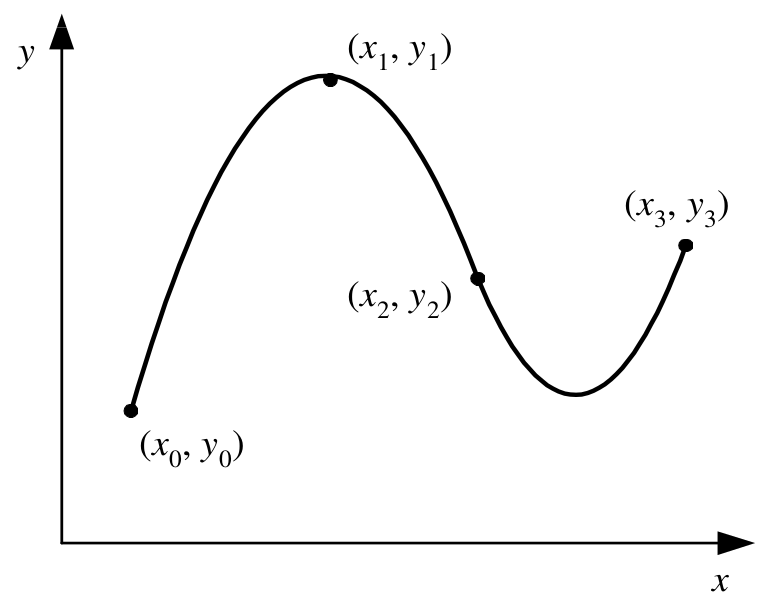
\includegraphics[width=0.4\linewidth]{img/img07}
		\end{center}
	\end{itemize}
\end{frame}

\begin{frame}{Interpolasi Kubik}
	Polinom $ p_3(x) $ ditentukan dengan cara berikut:
	\begin{enumerate}
		\item sulihkan $ (x_i, y_i) $ ke dalam persamaan \ref{int.kub} , $ i = 0, 1, 2, 3 $. Dari sini diperoleh empat buah persamaan dengan empat buah parameter yang tidak diketahui, yaitu $ a_0 $, $ a_1 $, $ a_2 $, dan $ a_3 $ :
		\begin{align*}
			a_0 + a_1 x_0 + a_2 x_0^2 + a_3 x_0^3 &= y_0 \\
			a_0 + a_1 x_1 + a_2 x_1^2 + a_3 x_1^3 &= y_1 \\
			a_0 + a_1 x_2 + a_2 x_2^2 + a_3 x_2^3 &= y_2 \\
			a_0 + a_1 x_3 + a_2 x_3^2 + a_3 x_3^3 &= y_3
		\end{align*}
		\item hitung $ a_0 $, $ a_1 $, $ a_2 $, dan $ a_3 $ dari sistem persamaan tersebut dengan metode eliminasi Gauss.
	\end{enumerate}
\end{frame}

\begin{frame}
	\begin{itemize}
		\item Dengan cara yang sama kita dapat membuat polinom interpolasi berderajat $ n $ untuk $ n $ yang lebih tinggi:
		\[ p_n(x) = a_0 + a_1 x + a_2 x^2 + \dots + a_n x^n \]
		asalkan tersedia $ (n+1) $ buah titik data.
		\item Dengan menyulihkan $ (x_i, y_i) $ ke dalam persamaan polinom di atas $ y = p_n(x) $ untuk $ i = 0, 1, 2, \dots, n $, akan diperoleh $ n $ buah sistem persamaan lanjar dalam $ a_0, a_1, a_2, \dots , a_n $,
		\begin{align*}
			a_0 + a_1 x_0 + a_2 x_0^2 + \dots + a_n x_0^3 &= y_0 \\
			a_0 + a_1 x_1 + a_2 x_1^2 + \dots + a_n x_1^3 &= y_1 \\
			&\vdots \\
			a_0 + a_1 x_n + a_2 x_n^2 + \dots + a_n x_n^3 &= y_n
		\end{align*}
		\item[] 
	\end{itemize}
\end{frame}

\begin{frame}
	\begin{itemize}
		\item Solusi sistem persamaan lanjar ini diperoleh dengan menggunakan metode eliminasi Gauss yang sudah anda pelajari.
		\item Secara umum, penentuan polinom interpolasi dengan cara yang diuraikan di atas kurang disukai,
		\item karena sistem persamaan lanjar yang diperoleh ada kemungkinan berkondisi buruk, terutama untuk derajat polinom yang semakin tinggi.
		\item Metode polinom interpolasi yang banyak digunakan dalam komputasi numerik adalah:
		\begin{enumerate}
			\item Polinom Lagrange
			\item Polinom Newton
			\item Polinom Newton-Gregory (kasus khusus dari polinom Newton)
		\end{enumerate}
	\end{itemize}
\end{frame}

\section{Polinom Lagrange}

\begin{frame}
	\frametitle{Polinom Lagrange}
	\begin{itemize}
		\item Tinjau kembali polinom lanjar:
		\[ p_1(x) = y_0 + \frac{(y_1 - y_0)}{(x_1 - x_0)}(x-x_0) \]
		\item Persamaan ini dapat diatur kembali sedemikian rupa sehingga menjadi
		\[ p_1(x) = y_0 + \frac{(x - x_1)}{(x_0 - x_1)} + y_1\frac{(x-x_0)}{(x_1-x_0)} \]
	\end{itemize}
\end{frame}

\begin{frame}{Polinom Lagrange}
	\begin{itemize}
		\item atau dapat dinyatakan dalam bentuk
		\[ p_1(x) = a_0 L_0 (x) + a_1 L_1 (x) \]
		\item yang dalam hal ini
		\[ a_0 = y_0,\quad L_0(x) = \frac{(x-x_1)}{(x_0-x_1)} \]
		dan
		\[ a_1 = y_1,\quad L_1(x) = \frac{(x-x_0)}{(x_1-x_0)} \]
	\end{itemize}
\end{frame}

\begin{frame}{Polinom Lagrange}
	\begin{itemize}
		\item Bentuk umum polinom Lagrange derajat $ \leq  n $ untuk $ (n + 1) $ titik berbeda adalah
		\begin{equation}\label{pol.lagr}
			p_n(x) = \sum_{i=0}^{n} a_i L_i(x) = a_0 L_0(x) + a_1 L_1(x) + \dots + a_n L_n(x)
		\end{equation}
		yang dalam hal ini
		\[ a_i = y_i,\quad i=0,1,2,\dots,n \]
		dan
		\begin{align*}
			L_i(x) &= \prod_{j=0;j\neq i}^{n} \frac{(x-x_j)}{(x_i-x_j)} \\
			&= \frac{(x-x_0)(x-x_1) \dots (x-x_{i-1})(x-x_{i+1})\dots (x-x_n)}{(x_i -x_0)(x_i-x_1) \dots (x_i-x_{i-1})(x_i-x_{i+1})\dots (x_i-x_n)}
		\end{align*}
	\end{itemize}
\end{frame}

\begin{frame}
	\frametitle{Contoh 4}
	\begin{itemize}
		\item \textbf{Persoalan:} Hampiri fungsi $ f(x) = \cos x $ dengan polinom interpolasi derajat tiga di dalam selang $ [0.0, 1.2] $. Gunakan empat titik, $ x_0 = 0.0 $, $ x_1 = 0.4 $, $ x_2 = 0.8 $, dan $ x_3 = 1.2 $. Perkirakan nilai $ p_3(0.5) $, dan bandingkan dengan nilai sejatinya.
		\item \textbf{Penyelesaian:}
		\begin{center}
			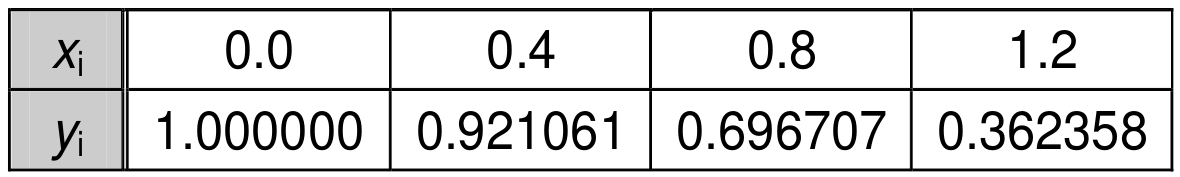
\includegraphics[width=0.7\linewidth]{img/img08}
		\end{center}
	\end{itemize}
\end{frame}

\begin{frame}{Contoh 4}
	\begin{itemize}
		\item Polinom Lagrange derajat 3 yang menginterpolasi keempat titik di tabel adalah
		\begin{align*}
			p_3 (x) &= a_0 L_0 (x) + a_1 L_1 (x) + a_2 L_2 (x) + a_3 L_3 (x) \\
			&= y_0 \frac{(x-x_1)(x-x_2)(x-x_3)}{(x_0-x_1)(x_0-x_2)(x_0-x_3)} \\
			&+ y_1 \frac{(x-x_1)(x-x_2)(x-x_3)}{(x_1-x_0)(x_1-x_2)(x_1-x_3)} \\
			&+ y_2 \frac{(x-x_1)(x-x_2)(x-x_3)}{(x_2-x_0)(x_2-x_1)(x_2-x_3)} \\
			&+ y_3 \frac{(x-x_1)(x-x_2)(x-x_3)}{(x_3-x_0)(x_3-x_1)(x_3-x_2)} \\
		\end{align*}
	\end{itemize}
\end{frame}

\begin{frame}{Contoh 4}
	\begin{itemize}
		\item[]
		\begin{align*}
		p_3 (x) &= 1.000000 \frac{(x-0.4)(x-0.8)(x-1.2)}{(0.0-0.4)(0.0-0.8)(0.0-1.2)} \\
		&+ 0.921061 \frac{(x - 0.0 )(x - 0.8)(x - 1.2)}{(0.4 - 0.0)( 0.4 - 0.8 )( 0.4 - 1.2 )} \\
		&+ 0.696707 \frac{(x - 0.0 )(x - 0.4)(x - 1.2)}{(0.8 - 0.0)( 0.8 - 0.4 )( 0.8 - 1.2 )} \\
		&+ 0.362358 \frac{(x - 0.0 )(x - 0.4)(x - 0.8)}{(1.2 - 0.0)( 1.2 - 0.4 )( 1.2 - 0.8 )} \\
		\end{align*}
	\end{itemize}
\end{frame}

\begin{frame}{Contoh 4}
	\begin{itemize}
		\item[]
		\begin{align*}
		p_3 (x) &= - 2.604167 ( x - 0.4 )( x - 0.8 )( x - 1.2 )
		&+ 7.195789 ( x - 0.0 )( x - 0.8 )( x - 1.2 ) \\
		&- 5.443021 ( x - 0.0 )( x - 0.4 )( x - 1.2 )\\
		&+ 0.943640 ( x - 0.0 )( x - 0.4 )( x - 0.8 )
		\end{align*}
	\end{itemize}
\end{frame}

\begin{frame}{Contoh 4}
	\begin{itemize}
		\item Untuk mengurangi galat akibat pembulatan, polinom $ p_3(x) $ ini tidak perlu disederhanakan lebih jauh. Kurva $ y = \cos(x) $ dan $ y = p_3(x) $ diperlihatkan pada Gambar berikut:
		\begin{center}
			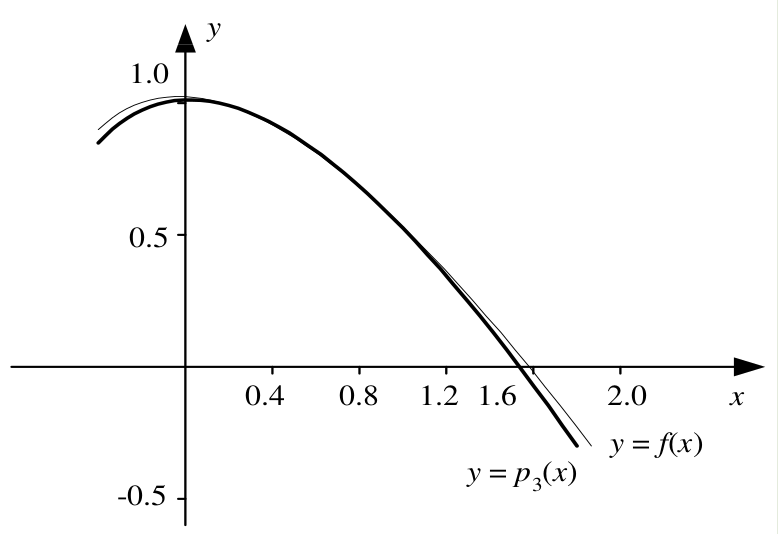
\includegraphics[width=0.7\linewidth]{img/img09}
		\end{center}
	\end{itemize}
\end{frame}

\begin{frame}{Contoh 4}
	\begin{itemize}
		\item Dengan menggunakan polinom interpolasi $ p_3 (x) $ itu kita dapat menaksir nilai fungsi di $ x = 0.5 $ sebagai berikut:
		\begin{align*}
			p_3(0.5) &= -2.604167(0.5 - 0.4)(0.5 - 0.8)(0.5 - 1.2) \\
			&+ 7.195789(0.5 - 0.0)(0.5 - 0.8)(0.5 - 1.2) \\
			&-5.443021(0.5 - 0.0)(0.5 - 0.4)(0.5 - 1.2) \\
			&+ 0.943640(0.5 - 0.0)(0.5 - 0.4)(0.5 - 0.8) \\
			&= 0.877221
		\end{align*}
		\item Sebagai perbandingan, nilai sejatinya adalah
		$ y = \cos(0.5) = 0.877583 $
	\end{itemize}
\end{frame}

\begin{frame}
	\frametitle{Contoh 5}
	\begin{itemize}
		\item \textbf{Persoalan:} Dari fungsi $ y = f(x) $, diberikan tiga buah titik data dalam bentuk tabel:
		\begin{center}
			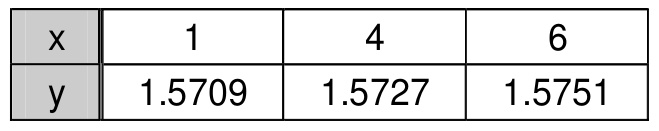
\includegraphics[width=0.7\linewidth]{img/img10}
		\end{center}
		Tentukan $ f(3.5) $ dengan polinom Lagrange derajat 2. Gunakan lima angka bena.
	\end{itemize}
\end{frame}

\begin{frame}{Contoh 5}
	\begin{itemize}
		\item \textbf{Penyelesaian:} Polinom derajat $ 2 \rightarrow n = 2 $ (perlu tiga buah titik)
		\[ p_2 (x) = L_0 (x) y_0 + L_1 (x) y_1 + L_2 (x) y_2 \]
	\end{itemize}
	\begin{align*}
		L_0(x) = \frac{( x - 4 )( x - 6 )}{( 1 - 4 )( 1 - 6 )} &\rightarrow L_0(3.5) = \frac{( 3 . 5 - 4 )( 3 . 5 - 6 )}{( 1 - 4 )( 1 - 6 )} = 0.083333 \\
		L_1(x) = \frac{( x - 1 )( x - 6 )}{( 4 - 1 )( 4 - 6 )} &\rightarrow L_1(3.5) = \frac{( 3 . 5 - 1 )( 3 . 5 - 6 )}{( 4 - 1 )( 4 - 6 )} = 1.0417 \\
		L_2(x) = \frac{( x - 1 )( x - 3 )}{( 6 - 1 )( 6 - 4 )} &\rightarrow L_2(3.5) = \frac{( 3 . 5 - 1 )( 3 . 5 - 4 )}{( 6 - 1 )( 6 - 4 )} = -0.12500 \\
	\end{align*}
		Jadi, $ p_2(3.5) = (0.083333)(1.5709) + (1.0417)(1.5727) + (-0.12500)(1.5751) = 1.5723 $
\end{frame}

\begin{frame}
	\frametitle{Komputasi Lagrange}
	\begin{itemize}
		\item Mari membuat algoritma dari Lagrange dan source code nya berbahasa Python
	\end{itemize}
\end{frame}




\end{document}
